\chapter{ELEMENTOS DO TEXTO}
\label{cap:elementos}

Graças ao grande numero de termos específicos da área de desenvolvimento, é necessária a explicação dos mesmos.

\section{Metodologias Ágeis}

\subsection{Scrum}

Metodologia ágil que visa ter escopo fechado(numero de tarefas predefinidas), calculadas através de métricas da equipe, como pontos de esforço.

Muitas vezes separadas em Sprints(tempo pre-definido pela equipe, geralmente de 10 dias utéis), as tarefas são incluídas em um quadro e devem ser finalizadas ate o fim do prazo.

\begin{quote}
  O framework Scrum consiste nos times do Scrum associadas a papéis, eventos, artefatos e
  regras. Cada componente dentro do framework serve a um propósito específico e é essencial
  para o uso e sucesso do Scrum.
\end{quote}

\subsection{Kanbam}
  Opção de metodologia ágil mais adaptativa, tendo escopo aberto torna-se possível inserir atividades durante o tempo.
  Geralmente se é determinado um máximo de esforço e ao final de alguma atividade, é inserida uma nova com prioridade.
\begin{figure}[!htb]
\centering
\caption{Quadro kanbam} %legenda
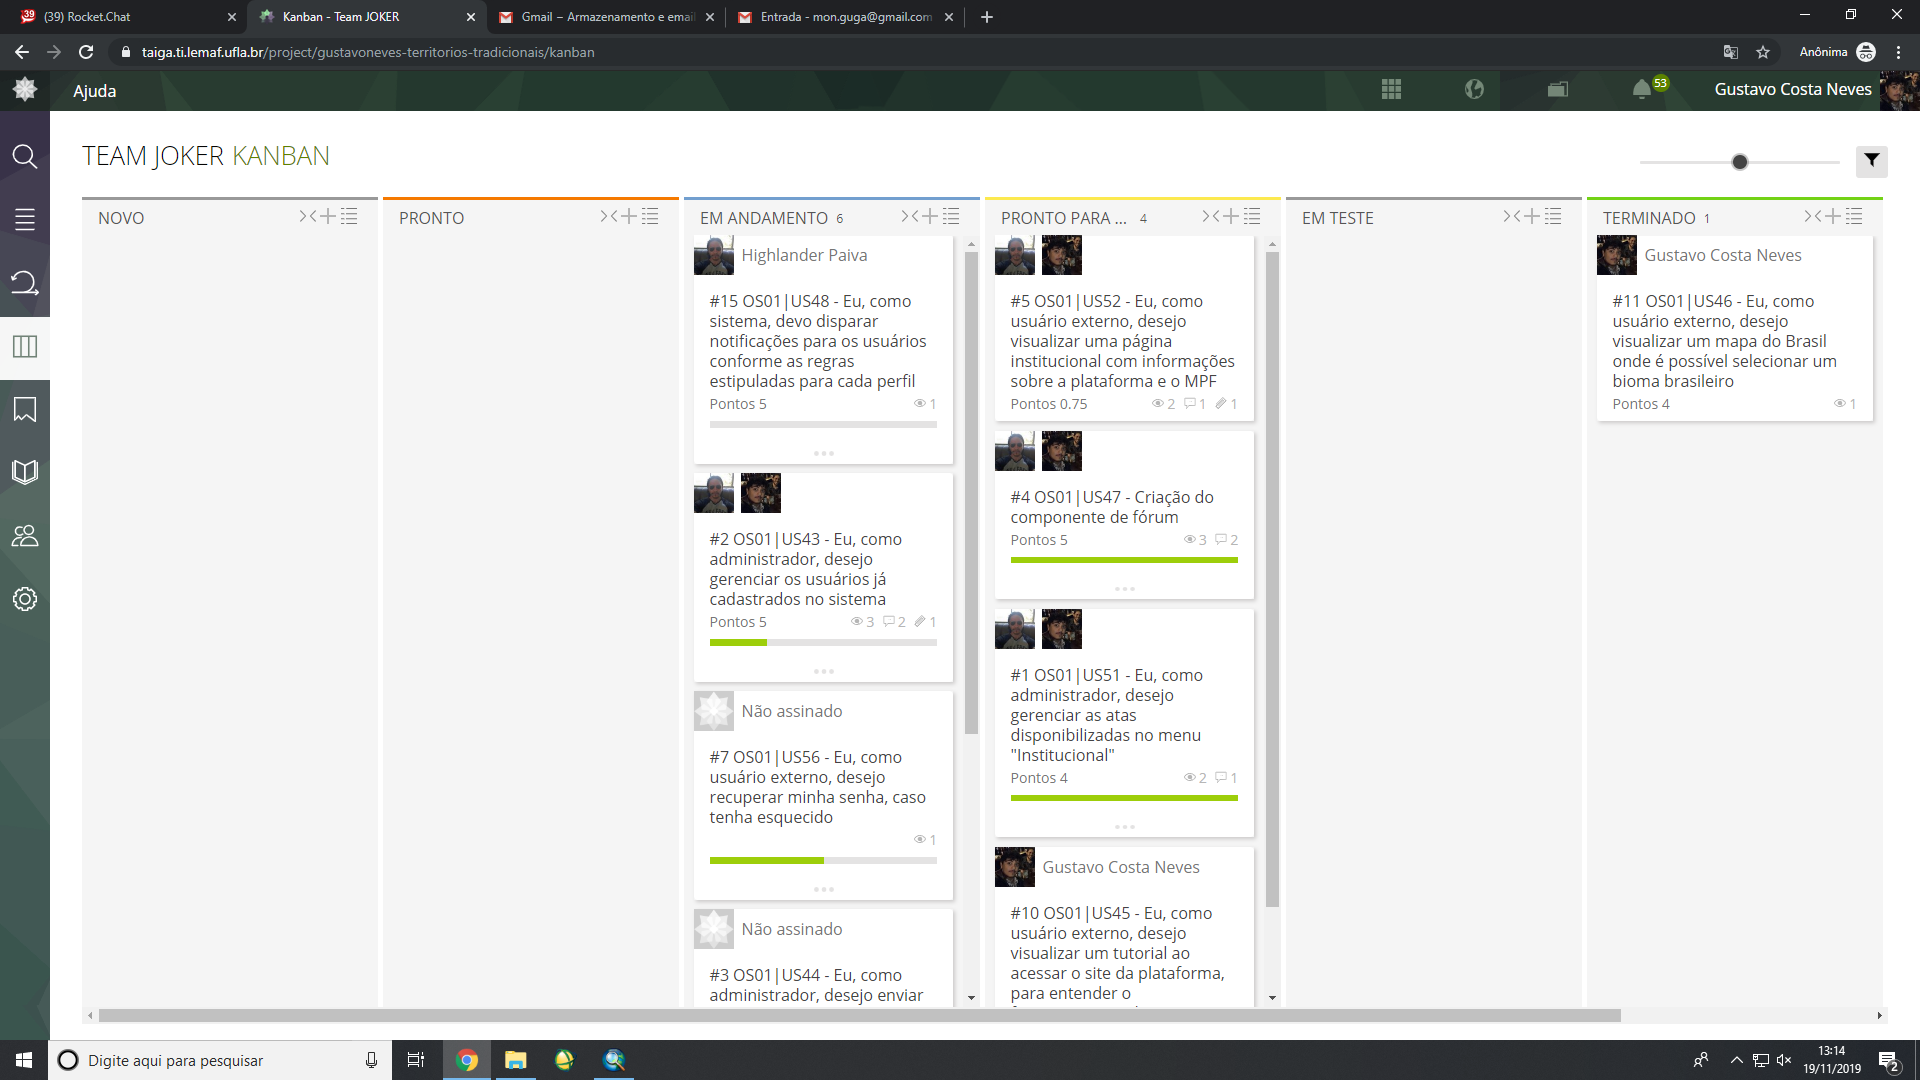
\includegraphics[scale=0.2]{quadroKanbam}\\  % o 0.9 indica 90% do tamanho original
% pdfLaTeX aceita figuras no formato PNG, JPG ou PDF
% figuras vetoriais podem ser exportadas para eps e depois convertidas para pdf usando epstopdf
{\small Fonte: https://taiga.ti.lemaf.ufla.br/} %Fonte da imagem
\label{fig:exemplo} %rotulo para refencia
\end{figure}

\section{Frameworks}

Para facilitar o desenvolvimento, diversas ferramentas já foram criadas e durante o desenvolvimento de novos projetos, foi necessária a utilização das mesmas.

\subsection{Frontend}

É a parte da aplicação que interage diretamente com o usuário.

\subsubsection{Angular}

Angular é um framework open-source de desenvolvimento front-end que possibilita o desenvolvimento de aplicações web.

Teve sua primeira versão foi lançada em 2016.

\subsubsection{VueJS}

Vue.js é um framework JavaScript de código-aberto, focado no desenvolvimento de interfaces de usuário e aplicativos de página única

Teve sua primeira versão lançada em 2014.

\subsubsection{ReactJS}

O React é uma biblioteca JavaScript de código aberto com foco em criar interfaces de usuário em páginas web. É mantido pelo Facebook, Instagram, outras empresas e uma comunidade de desenvolvedores individuais. 

Teve sua primeira versão lançada em 2013.

\subsection{Backend}

É a parte da aplicação que fica escondida do usuário, é onde é controlado todo o sistema(autenticação, regras de negocio, jobs e etc).

\subsubsection{PlayFramework}

O Play Framework é uma alternativa "limpa" de esticar as stacks do Java Enterprise. Ele se concentra na produtividade do desenvolvedor e tem como objetivo arquiteturas RESTful. O Play é um companheiro perfeito para o desenvolvimento ágil de software.

O objetivo da estrutura do Play é facilitar o desenvolvimento de aplicativos da web, mantendo o Java.

Teve sua primeira versão lançada em 2009.

\subsubsection{Spring Boot}

O Spring é um framework open source para a plataforma Java criado por Rod Johnson e descrito em seu livro "Expert One-on-One: JEE Design e Development". Trata-se de um framework não intrusivo, baseado nos padrões de projeto inversão de controle e injeção de dependência.

Teve sua primeira versão em 2002.

\subsubsection{DotNet Framework}

O .NET Framework é uma iniciativa da empresa Microsoft, que visa uma plataforma única para desenvolvimento e execução de sistemas e aplicações. Todo e qualquer código gerado para .NET pode ser executado em qualquer dispositivo que possua um framework de tal plataforma.

Teve sua primeira versão lançada em 2002.

\section{Cargos}

Para melhor organização dos projetos, os funcionários são separados em tribos e squads com alguns cargos específicos para cada integrante.

\subsection{Scrum Master}

Cargo que tem como função cuidar das obrigações impostas sobre a metodologia scrum, como lembrar dos ritos, marcar reuniões, desimpedir atividades.

\subsection{Gerente de projetos(GP)}

Cargo que tem como função gerenciar os projetos e times da sua
 tribo, cuidando para que sejam entregue os requisitos no prazo combinado.

\subsection{Product Owner(PO)}
Cargo que tem como função cuidar do relacionamento do time com o produto,
 definindo e priorizando requisitos.